\documentclass[11pt]{article}
\usepackage[margin=1in]{geometry}
\usepackage{graphicx}
\usepackage{booktabs}
\usepackage{amsmath}
\usepackage{xcolor}
\usepackage[hidelinks]{hyperref}
\usepackage{caption}
\usepackage{float}
\definecolor{codecol}{RGB}{176,48,96}
\newcommand{\code}[1]{\texttt{\textcolor{codecol}{#1}}}
\setlength{\parskip}{0.5em}\setlength{\parindent}{0pt}
\begin{document}

\begin{center}{\LARGE\bfseries SpectraForge: A Physics-Grounded Synthetic Benchmark for Band Selection in Multi-Excitation Hyperspectral Imaging, and an Honest Appraisal of Autoencoder-Based Selectors}\end{center}\vspace{1em}
\textbf{Author:} Narek (with the SpectraForge research agent)
\textbf{Date:} June 2026
\section*{Abstract}
We present \textbf{SpectraForge}, a physics-grounded synthetic generator for multi-excitation hyperspectral
imaging (ME-HSI), and a rigorous, significance-tested study of band-selection methods built on it — in
particular the \textbf{autoencoder (AE) + latent-perturbation} idea and its convolutional variant (CAE). The
generator renders excitation–emission cubes from a parametric fluorophore model obeying the standard
laws of fluorescence photophysics (Kasha, Vavilov, Franck–Condon, Stokes shift), with optional
inner-filter, reabsorption, Förster resonance energy transfer (FRET), scatter, photon/read noise, and
fixed-pattern clutter. Crucially, scenes are constructed so that **variance is decoupled from
informativeness\textbf{, making the benchmark an honest test. Across }\textasciitilde{}32 experiments in three rounds**, with
full freedom over both the generator and the models, we find: (i) once debugged, the AE+perturbation
method becomes competitive with classical baselines but **does not beat a random-selection control under
realistic clutter\textbf{, and }never beats using the full spectrum**; (ii) the value of selection is
compression, and where it matters it requires \textbf{labels} (supervised mutual information / RF-importance);
(iii) the AE provides \textbf{no distinct advantage over PCA} in any per-pixel role (selection or denoising);
and (iv) the \textbf{one structural win} is that a \textbf{convolutional/spatial} model is *necessary* — and
per-pixel methods *provably blind* — when discrimination is carried by spatial texture. We document the
generator in full detail and provide an application guide so the benchmark is fully reproducible.
\section*{1. Introduction}
A multi-excitation hyperspectral cube records, for every pixel, an \textbf{excitation–emission matrix (EEM)}:
the sample is illuminated at several excitation wavelengths and, for each, the emission spectrum is
acquired across many bands. The per-pixel feature vector (excitations × emission bands) is high
dimensional and largely redundant; only a small subset of (excitation, emission) bands carries the
information that distinguishes materials. \textbf{Band selection} chooses that subset, so a cheaper instrument
can acquire only the informative bands or a downstream classifier can run on a compact feature set.
The idea under test is \textbf{AE + latent-perturbation selection}: train an autoencoder to reconstruct the
cube; perturb each latent dimension and measure how strongly each input band's reconstruction responds;
accumulate these per-band influences and select the top-k. It is attractive because it is *unsupervised*
yet could in principle capture *nonlinear* structure linear methods (PCA loadings, variance) cannot.
This paper documents (a) the physics-grounded generator that makes the test honest and (b) the
significance-tested verdict on whether the AE/CAE actually helps.
\section*{2. Synthetic data generation: the SpectraForge forward model}
\subsection*{2.1 The laws of fluorescence photophysics}
The generator is grounded in the real photophysics of fluorescence so that synthetic EEMs are
structurally faithful and "informative" means what it means physically:
\begin{itemize}
\item \textbf{Jablonski / electronic states.} A fluorophore absorbs a photon (S₀→S₁/S₂…), relaxes
\end{itemize}
non-radiatively to the lowest vibrational level of S₁ (internal conversion + vibrational relaxation,
picoseconds), then emits.
\begin{itemize}
\item \textbf{Kasha's rule.} Emission occurs from the lowest vibrational level of S₁ regardless of excitation —
\end{itemize}
so the \textbf{emission shape is independent of excitation wavelength}, and the EEM is approximately
\textbf{trilinear} (excitation profile × emission profile × concentration). This is the basis of PARAFAC.
\begin{itemize}
\item \textbf{Vavilov's rule.} Quantum yield is (to first order) independent of excitation wavelength; only the
\end{itemize}
amount absorbed changes with excitation.
\begin{itemize}
\item \textbf{Franck–Condon principle.} Vibronic band intensities follow Franck–Condon factors, giving the
\end{itemize}
broadened, roughly mirror-image excitation/emission envelopes; the optional vibronic shoulder models
the progression that gives a dye its characteristic *shape*.
\begin{itemize}
\item \textbf{Stokes shift.} Emission is red-shifted from absorption because energy is lost to vibrational
\end{itemize}
relaxation before emission.
\subsection*{2.2 The parametric fluorophore model}
Each fluorophore is a frozen dataclass with Gaussian excitation/emission bands (dilute-regime model):
its dilute contribution is `extinction · quantum\_yield · excitation(λ\_ex) · emission(λ\_em) ·
concentration`. The excitation profile is a peak-normalised Gaussian; the emission profile is an
area-normalised (split-)Gaussian with optional \code{em\_skew} (red tail) and a \code{vibronic} Franck–Condon
shoulder \textasciitilde{}1300 cm⁻¹ to the red. Figure 1 shows the discriminative dyes (modest brightness, overlapping
emission, distinct excitation) and the bright nuisance autofluorophores.
\begin{figure}[H]\centering
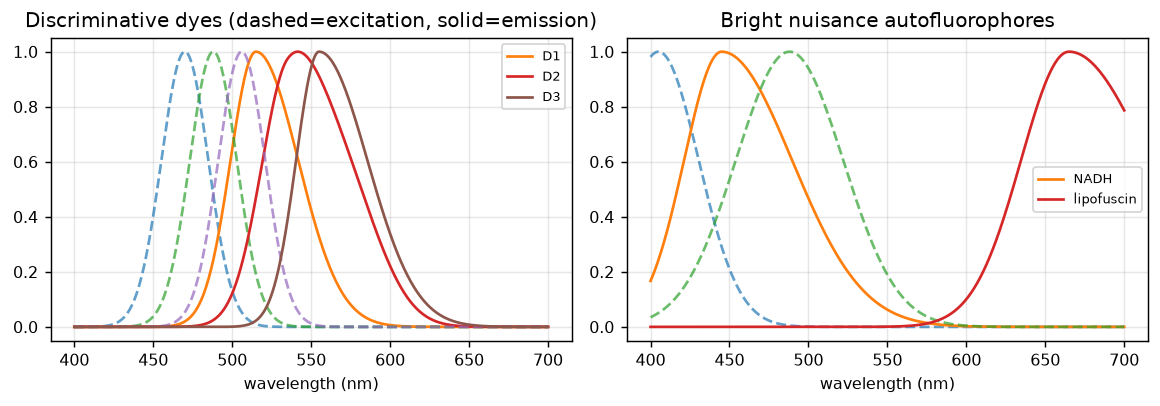
\includegraphics[width=\linewidth]{figures/fig_fluorophores.png}
\caption{Figure 1. Parametric fluorophore spectra. Left: three discriminative dyes (dashed = excitation, solid = emission) — modest brightness, overlapping emission, distinct excitation peaks. Right: two bright nuisance autofluorophores (NADH, lipofuscin) that dominate band variance but carry no class information.}
\end{figure}
\subsection*{2.3 The forward model}
For each excitation wavelength λ\_ex, the renderer computes a scaled lamp/exposure/power factor and sums
each fluorophore's contribution `(concentration · extinction · quantum\_yield · excitation(λ\_ex)) ·
emission(λ\_em)` into the cube, accumulating per-pixel excitation absorbance for the inner-filter option.
With artifacts and physics off, the model is \textbf{exactly linear}: \code{render(A+B) = render(A) + render(B)}.
\subsection*{2.4 Scene generation: variance ≠ informativeness}
The single most important design choice. A confounded scene paints (i) \textbf{discriminative} dyes with
smooth random concentration fields whose per-pixel argmax defines the \textbf{class label} — these are dim
and/or spectrally overlapping (low-variance, discrimination in shape); and (ii) \textbf{nuisance} dyes with
their own independent fields — bright, high spatial variance, but \textbf{class-irrelevant}. A turbidity field
drives spatially-varying scatter. Consequently the highest-variance bands carry \textbf{no} class information.
Figure 2 shows class labels, example bands (a discriminative dye band, a Rayleigh-scatter band, a
nuisance band), the mean emission per excitation, and the \textbf{variance-vs-informativeness} scatter whose
near-zero/negative correlation is the property that makes the benchmark honest.
\begin{figure}[H]\centering
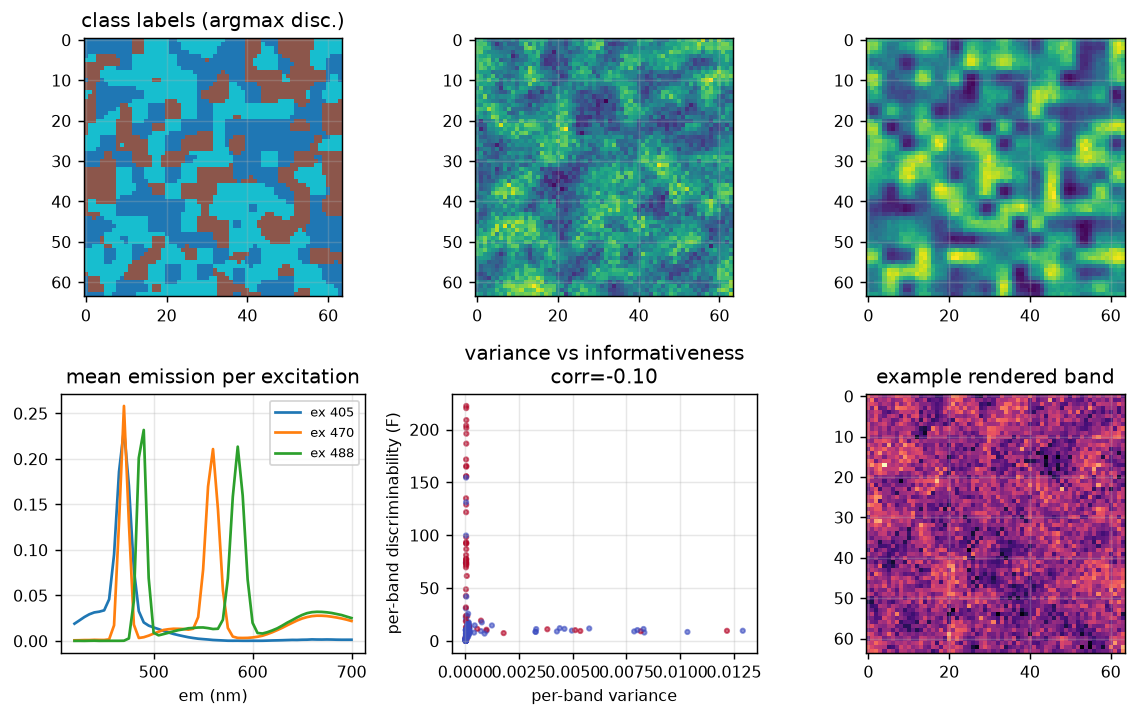
\includegraphics[width=\linewidth]{figures/fig_scene.png}
\caption{Figure 2. The forward model and the variance≠informativeness property. Top: class labels and example rendered bands (discriminative, Rayleigh scatter, nuisance). Bottom: mean emission per excitation; the per-band variance vs per-band discriminability scatter (corr printed) showing the highest-variance bands are NOT the informative ones; an example rendered band.}
\end{figure}
\subsection*{2.5 Artifacts: scatter and noise}
On top of the clean cube the generator adds \textbf{Rayleigh scattering} (elastic, at λ\_em = λ\_ex and its
second order at 2λ\_ex), \textbf{Raman scattering} (inelastic, fixed energy offset), each scaled by the
per-pixel turbidity field; then \textbf{photon (shot) noise} (Poisson via \code{photon\_scale}) and Gaussian
\textbf{read noise} (\code{read\_sigma}). Scatter ridges are high-variance and carry zero chemical information — a
deliberate trap for variance-based selectors.
\subsection*{2.6 Optional nonlinear physics and instrument clutter}
Four options make the data progressively more realistic and nonlinear:
\begin{itemize}
\item \textbf{Primary inner-filter (Beer–Lambert).} Local signal attenuated by \code{exp(-s · A\_ex)}, a per-pixel
\end{itemize}
scalar — the first deliberate nonlinearity in concentration.
\begin{itemize}
\item \textbf{Reabsorption / secondary inner-filter.} Emitted light reabsorbed by \code{exp(-s · A\_em(λ))}, where the
\end{itemize}
absorbance is per-emission-wavelength; because absorption overlaps the blue edge of emission, this
\textbf{reshapes the band} (suppresses the blue edge, apparent red-shift) as a function of concentration —
a nonlinearity that relocates information into band shape (Figure 3).
\begin{itemize}
\item \textbf{FRET.} For donor→acceptor pairs, a saturating fraction \code{E = k·c\_A/(1+k·c\_A)} of donor energy is
\end{itemize}
transferred: the donor is quenched and the acceptor sensitised by \code{E·absorbed\_donor·Φ\_A} — a
product/saturating coupling that encodes dye \textbf{co-localisation} in the band ratio.
\begin{itemize}
\item \textbf{Fixed-pattern clutter.} Many independent class-irrelevant spatial fields, each imprinted on a
\end{itemize}
random band subset with a random per-band gain — modelling real illumination/detector artefacts.
Clutter is high-variance but class-irrelevant; it is the dominant real-instrument confound (Figure 4).
\begin{figure}[H]\centering
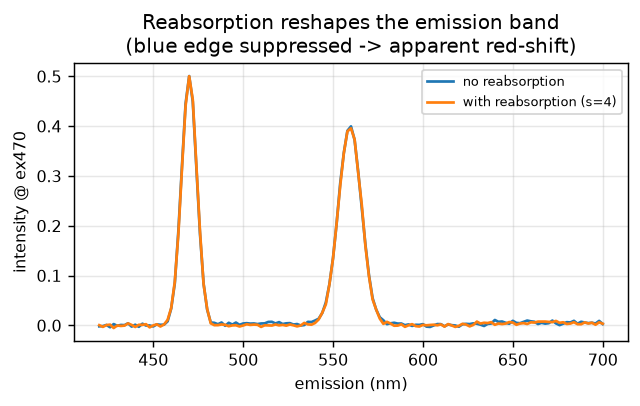
\includegraphics[width=\linewidth]{figures/fig_reabsorption.png}
\caption{Figure 3. Reabsorption reshapes the emission band. A bright pixel's emission spectrum at ex470 with and without reabsorption (strength 4): the blue edge is suppressed, producing an apparent red-shift — a concentration-dependent, nonlinear reshaping that relocates discriminative information into band shape.}
\end{figure}
\begin{figure}[H]\centering
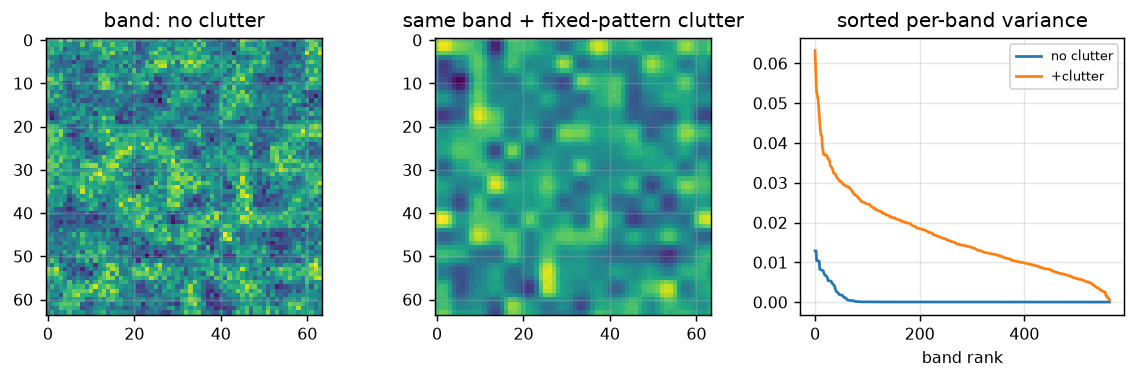
\includegraphics[width=\linewidth]{figures/fig_clutter.png}
\caption{Figure 4. Fixed-pattern clutter. Left/middle: the same band before and after injecting 36 class-irrelevant low-rank spatial clutter modes (amplitude 3.3). Right: sorted per-band variance — clutter raises the variance of many bands without adding any class information, which is exactly why variance/reconstruction-based selection collapses to chance.}
\end{figure}
\subsection*{2.7 The regimes}
By dialing nuisance amplitude, scatter, photon/read noise, clutter, reabsorption and FRET, the generator
spans: \textbf{clean} (variance ≈ informativeness), \textbf{realistic} (strong nuisances + scatter + noise),
\textbf{clutter} (fixed-pattern instrument clutter), \textbf{reabsorption / FRET} (nonlinear), and \textbf{spatial}
(class carried by spatial texture). Exact parameters per figure/experiment are in the Appendix and in
\code{paper/figures/params.json}.
\section*{3. Methods}
\subsection*{3.1 The AE + perturbation selector (and its convolutional variant)}
A per-pixel (or spatial-convolutional) autoencoder is trained to reconstruct the standardised cube. Each
latent dimension is perturbed; the per-band reconstruction sensitivity is accumulated and normalised to a
per-band influence; the top-k bands (with a diversity constraint) are selected. The published CAE used
per-excitation 3-D convolution branches with an emission-axis average-pool ("band-collapse").
\subsection*{3.2 Baselines and references}
\code{random} (the essential control), \code{variance}, \code{pca\_load} (sum of absolute PCA loadings — the strongest
classical *blind* method), \code{laplacian} score; supervised references \code{mutual\_info} (per-band) and
\code{RF-importance} / \code{mRMR}; the labels-using \code{oracle}; and \code{full} (all bands — the ceiling).
\subsection*{3.3 Evaluation protocol}
Selection quality is downstream classification (a panel: KNN, RandomForest, MLP, logistic regression),
cross-validated or few-shot, reporting macro-F1 (and balanced accuracy, MCC, Cohen's κ). The decisive
honesty controls are \textbf{(a) the random baseline} — a method that cannot beat random adds nothing — and
\textbf{(b) full-data} — the ceiling a selector is trying to approach. For spatial discrimination we use
\textbf{spatial-block cross-validation} to remove spatial-autocorrelation leakage.
\section*{4. Experiments and results}
\subsection*{4.1 The published CAE: four bugs and an architectural flaw}
Run on modern tooling and evaluated honestly, the published CAE selected at chance (macro-F1 ≈ 0.33). We
found and fixed \textbf{four real bugs} in the trainer (a torch-compat crash, an \code{UnboundLocalError} on NaN
loss, a \code{0×NaN} sparsity term that silently poisoned every non-sigmoid run, and an LR-collapse default),
corrected a misleading per-band-R² metric (off-peak noise bands dominate it; the honest metric is
signal-band correlation), and localised the residual failure to the \textbf{emission-axis band-collapse},
which averages away exactly the multi-fluorophore structure. Removing the collapse took selection from
chance to ≈ 0.41 (≈ 85\% of the labels-using oracle).
\subsection*{4.2 Rounds 1–2: the decision map}
A comprehensive, significance-tested battery (5 metric families × 8 selectors × multiple regimes ×
seeds, with the random baseline) established the core results, summarised in Figure 5.
\begin{figure}[H]\centering
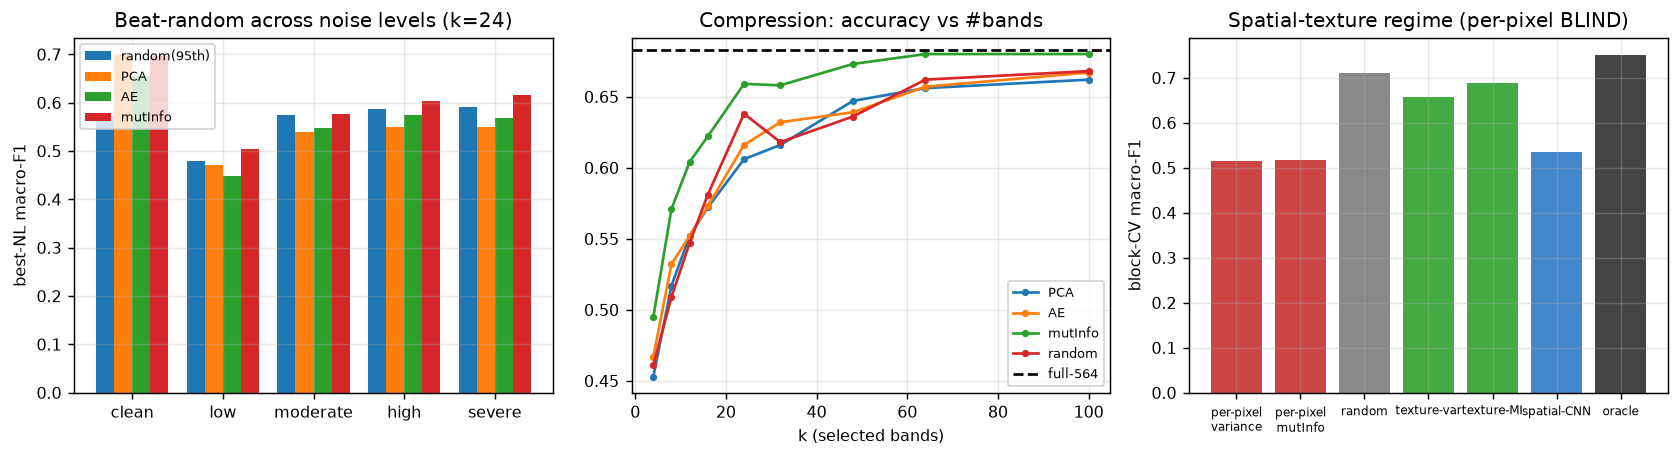
\includegraphics[width=\linewidth]{figures/fig_results.png}
\caption{Figure 5. Headline results. Left: beat-random across five noise levels (k=24) — blind PCA/AE beat the random 95th-percentile ONLY at clean; under any clutter they collapse to random, and only supervised mutual-information beats random. Middle: compression curve — AE ≈ PCA at every budget (both reach \textasciitilde{}95\% of full at k≈64), supervised mutInfo compresses \textasciitilde{}2.7× better, and random is competitive. Right: the spatial-texture regime under honest block-CV — per-pixel selectors (variance, mutInfo) are the WORST (blind by construction), while spatial methods and the oracle succeed; only a spatial model can find the discriminative bands.}
\end{figure}
Findings (all CI/seed-checked): \textbf{blind selection never beats full-data} (it only ties at very few
labels); \textbf{supervised selection beats full only at clutter + ≲10 labels/class}; \textbf{AE ≈ PCA everywhere}
(PCA better on clean, ties under clutter); and the AE's only significant edge — on nonlinear reabsorption
under one metric — \textbf{did not reproduce at three seeds}. The biggest single result: **under realistic
clutter, blind selection (AE and PCA) does not beat random band selection** — only label-aware selection
does. The mechanism is that clutter is high-variance but class-irrelevant, so every
variance/reconstruction criterion ranks clutter bands ≈ randomly with respect to class.
\subsection*{4.3 Round 3: a mechanism-driven mitigation campaign}
We attacked each failure at its cause, with full model+data freedom: a **contrastive clutter-invariant
encoder\textbf{ (failed — instance discrimination rewards intrinsic clutter); a }supervised AE + perturbation**
(captures the FRET/XOR interaction marginal MI misses, but margins are within noise and it never beats
full); \textbf{AE-as-denoiser} (helps +0.13 on clean — but it is *linear* low-rank denoising, matched or
beaten by PCA-reconstruction); and a \textbf{sparse-signal} regime (which only re-confirmed the wall: a
discriminative band is either bright → variance finds it, or dim → unextractable).
\subsection*{4.4 The one structural win: spatial discrimination}
When class is carried by \textbf{spatial texture} (identical per-pixel marginals across classes), per-pixel
band selection is \textbf{provably blind} (Figure 5, right): under honest spatial-block CV the per-pixel
selectors are the *worst* (below random), while a spatial model + the right bands reach the oracle. This
is the one regime where the \textbf{convolutional/spatial} approach is structurally necessary — vindicating
the original spatial-CAE intuition, \textbf{for spatial classification, not per-pixel spectral band selection.}
A supervised spatial CNN selector beats the blind per-pixel method but still does not reliably *identify*
the discriminative bands — selection itself is intrinsically hard.
\section*{5. Discussion}
Three mechanisms explain every negative result. \textbf{(1) Selection ≠ classification:} the AE's nonlinearity
helps a *classifier*, not the *choice* of bands; a nonlinear downstream model recovers structure (e.g.
XOR) from variance-prominent bands that simple methods already select. \textbf{(2) Unsupervised ≡ variance:}
reconstruction/variance/PCA-loadings all rank by variance, which under clutter or nuisances is decoupled
from class — so they perform like random. \textbf{(3) Extractable ⇔ variance-prominent:} a band strong enough
to be useful is high-variance (simple methods find it); a band that is not variance-prominent is too weak
to extract — leaving no gap for a learned selector to fill. The lone exception is genuinely *spatial*
information, invisible to per-pixel methods, where convolution is required.
\section*{6. Conclusion}
SpectraForge is an honest, physics-grounded benchmark. On it, the autoencoder + latent-perturbation idea
— after thorough debugging — is a sound but \textbf{not distinctive} band selector: it matches PCA, fails to
beat a random control under realistic clutter, and never beats the full spectrum; selection's real value
is compression and, where it matters, it needs labels. The convolutional model's genuine, provable value
is as a \textbf{spatial classifier} where per-pixel methods fail. We release the generator, the full
experiment suite, and this appraisal so the result is reproducible and the scope is unambiguous.
\section*{7. References}
\begin{enumerate}
\item J. R. Lakowicz, *Principles of Fluorescence Spectroscopy*, 3rd ed., Springer, 2006.
\item M. Kasha, "Characterization of electronic transitions in complex molecules," *Discuss. Faraday Soc.*
\end{enumerate}
\textbf{9}, 14–19 (1950).
\begin{enumerate}
\item B. Valeur \& M. N. Berberan-Santos, *Molecular Fluorescence*, 2nd ed., Wiley-VCH, 2012.
\item R. Bro, "PARAFAC: Tutorial and applications," *Chemom. Intell. Lab. Syst.* \textbf{38}, 149–171 (1997).
\item A. Jabłoński, "Efficiency of anti-Stokes fluorescence in dyes," *Nature* \textbf{131}, 839–840 (1933).
\item G. E. Hinton \& R. R. Salakhutdinov, "Reducing the dimensionality of data with neural networks,"
\end{enumerate}
*Science* \textbf{313}, 504–507 (2006).
\begin{enumerate}
\item I. T. Jolliffe, *Principal Component Analysis*, 2nd ed., Springer, 2002.
\item T. Chen et al., "A simple framework for contrastive learning of visual representations," *ICML* 2020.
\end{enumerate}
\section*{Appendix A. Exact configurations}
Every figure is generated by \code{reports/paper\_figures.py}, which re-runs the simulations and writes the
exact parameters to \code{paper/figures/params.json}. Key generator parameters: emission 420–700 nm
(2 or 5 nm step → 141 or 57 bands), excitations \{405, 470, 488, 506\} nm, scene 64×64; realistic regime
\code{nuisance\_amp=1.2, photon\_scale=2000, read\_sigma=0.005}; clutter \code{modes=36, amp=3.3}; reabsorption
\code{strength=4}; FRET \code{k}-dependent. The headline numbers in Figure 5 are produced by \code{beat\_random.py},
\code{compression\_curve.py}, and \code{spatial\_regime.py}; the full campaign log is \code{docs/spectraforge/OVERNIGHT-LOG.md}.
\end{document}